\chapter{Resultats}
\label{chap-results}

\section{État fondamental du calcium oxalate}
Les calculs numériques qui seront présentés dans cette section sont faits avec \textit{Abinit}.

\subsection{Structure moléculaire}
La cellule élémentaire de l'oxalate de calcium ($\V{Ca} \V{C}_2 \V{O}_4$) contient 28 atomes.
Il est de structure monoclinique et de groupe de symétrie $P2/m$ ($\#$10)~\cite{Kolezynski2010} (cf. \cref{BrillouinZone}).

\begin{figure}[!h]
  \centering
  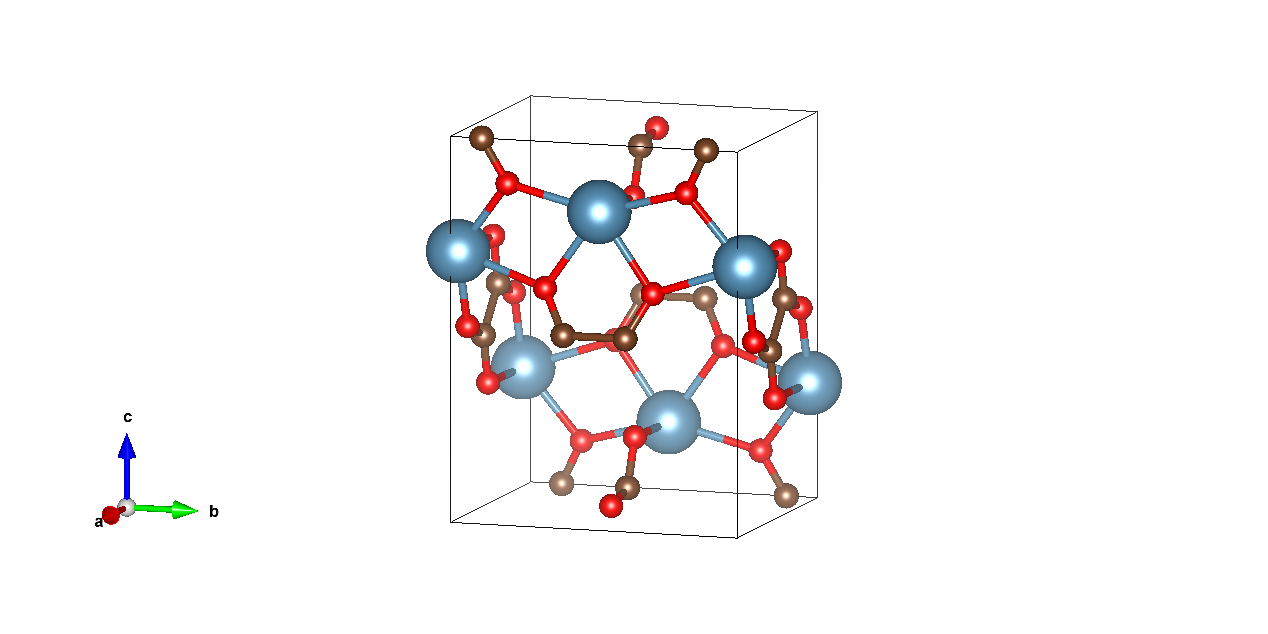
\includegraphics[height=0.4\textheight]{co_structure}
  \caption{La cellule élémentaire de l'oxalate de calcium avec $\V{Ca}$ en bleu, $\V{O}$ en rouge et $\V{C}$ en marron.}\label{BrillouinZone}
\end{figure}

\subsection{Energie de seuil}
D'abord, nous avons calculé la densité d'électrons de l'état fondamental
à l'aide des fonctions d'onde de Kohn et Sham,
qui sont elles-même représentées dans l'espace d'ondes planes tranché.
Pour chaque échantillonnage, l'énergie totale du système à l'état fondamental a été calculée
en variant $E_{\V{cut}}$ (cf. \cref{subsec-planewave}).
Le but du jeux est d'assurer la convergence du calcul en prenant le moins de fonctions d'onde possible.
Nous avons fait varier le seuil d'énergie $E_{cut}$ entre 20 et 100 Hatree.
La relation entre l'énergie totale du système à la convergence
en fonction de l'énergie de seuil est tracée dans la \cref{fig-Ecut}.
À partir de $E_{cut} = 40$ Hatree, l'énergie totale du système est bien minimisée.
Nous avons choisi donc cette énergie de seuil pour la suite du calcul de l'état fondamental.

\begin{figure}[!h]
    \centering
    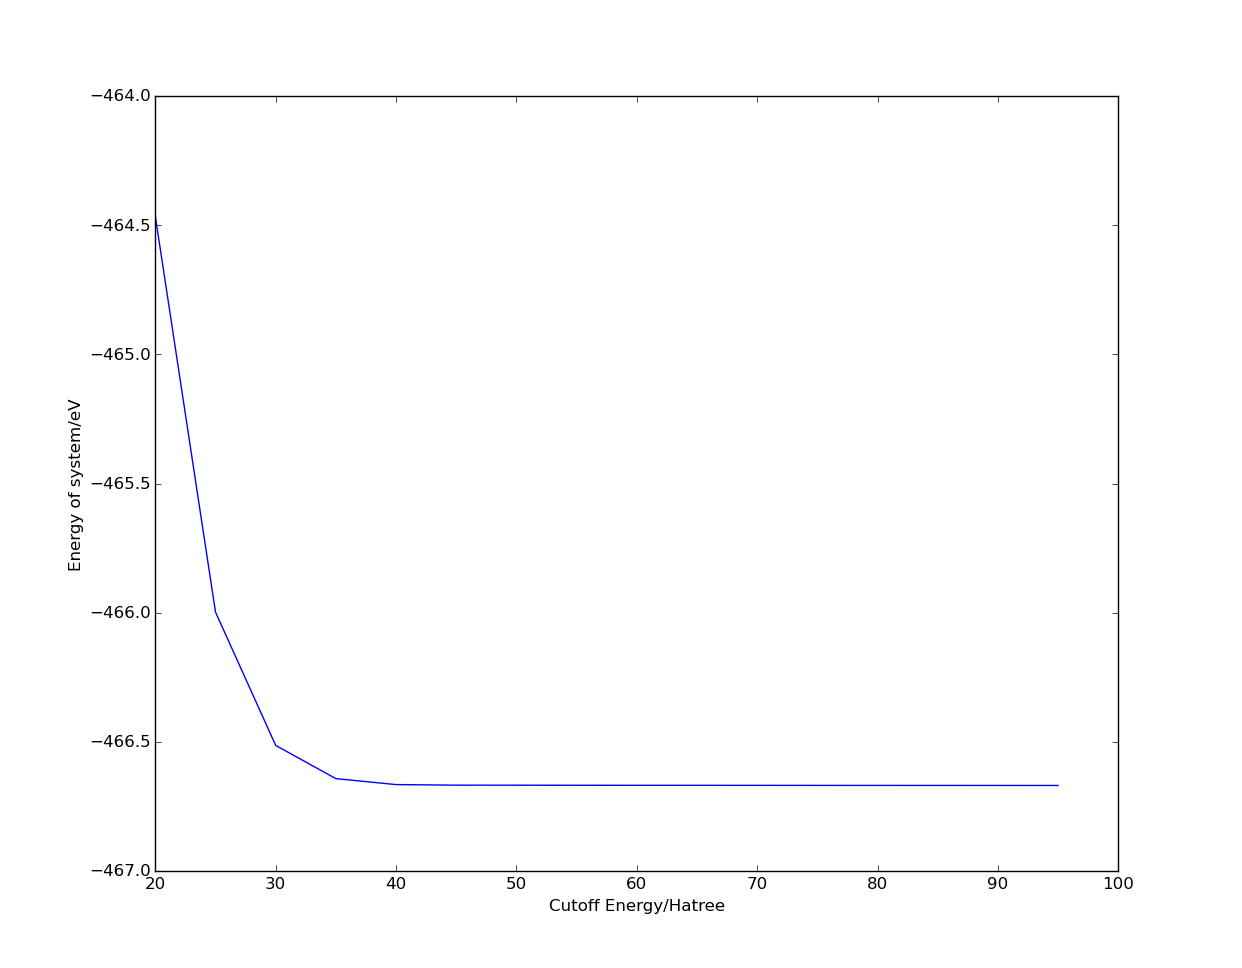
\includegraphics[width=\textwidth]{E_cut}
    \caption{L'énergie totale du système (en eV) en fonction de l'énergie de seuil (en Hatree).}\label{fig-Ecut}
\end{figure}

\subsection{Convergence avec les points-$\vb{k}$: I}
Etant donnée la structure du système étudié et une fonction d'essai dont l'intégrale est facile à calculer,
Abinit peut nous donner une liste des échantillonnages pertinents pour la structure du matériau.
La motivation de ce test de convergence est de pouvoir avoir un échantillonnage
assez fin pour obtenir tous les états d'excitation possibles sans avoir trop de points-$\vb{k}$,
ce qui augmentera considérablement la compléxité du calcul.

Le \cref{tab-etotPK} montre que le système converge déjà avec peu de points-$\vb{k}$ (16) dans la première zone de Brillouin.
Ce résultat est dû au fait que la première zone de Brillouin est petite (car la maille élémentaire est grande).
\begin{table}[ht]
  \captionsetup{width=0.6\textwidth}
  \caption{Énergie totale du système\\ en fonction du nombre de points-$\vb{k}$}\label{tab-etotPK}
  \centering
  \begin{tabular}{c c}
    \toprule
    Nombre de points-$\vb{k}$  &  $E_{\V{tot}}$ à la convergence (Hatree)
    \\
    \midrule
    16    &  -466.66501448840
    \\
    28    &  -466.66501224916
    \\
    40    &  -466.66501098806
    \\
    \bottomrule
  \end{tabular}
\end{table}
\section{Spectres de perte d'énergie (EELS)}
Les calculs de cette section sont faits avec le code de \textit{DP}.
L'objectif de cette section est de présenter les caractéritiques spectroscopiques
auxquelles on peut s'attendre dans une vraie expérience.

\subsection{Convergence avec les points-$\vb{k}$: II}
Bien que les calculs de convergence avec les nombres de points-$\vb{k}$ différents aient été faits pour l'état fondamental,
il faut s'assurer que l'échantillonnage que l'on a privilégié soit aussi assez fin pour calculer la réponse du matériau sous une excitation externe.
Nous avons créé des fichiers décrivant la densité de l'état fondamental avec des échantillonnages
de la première zone de Brillouin différents,
où dans la première zone de Brouillin, il y a respectivement 16, 120 et 480 points-$\vb{k}$.
Pour connaître le meilleur échantillonnage à utiliser à notre disposition,
on fait d'abord les calculs en prenant RPA (random phase approximation)
comme méthode d'approximation du terme d'échange et de corrélation.
Pour le cas de l'oxalate de calcium, nous avons choisi dans cette liste trois échantillonnages,
qui contiennent respectivement 16 (avec symétries),
120 (avec symétries) et 480 (grillage translaté et sans symétries) points-$\vb{k}$.

\begin{figure}[!h]
    \centering
    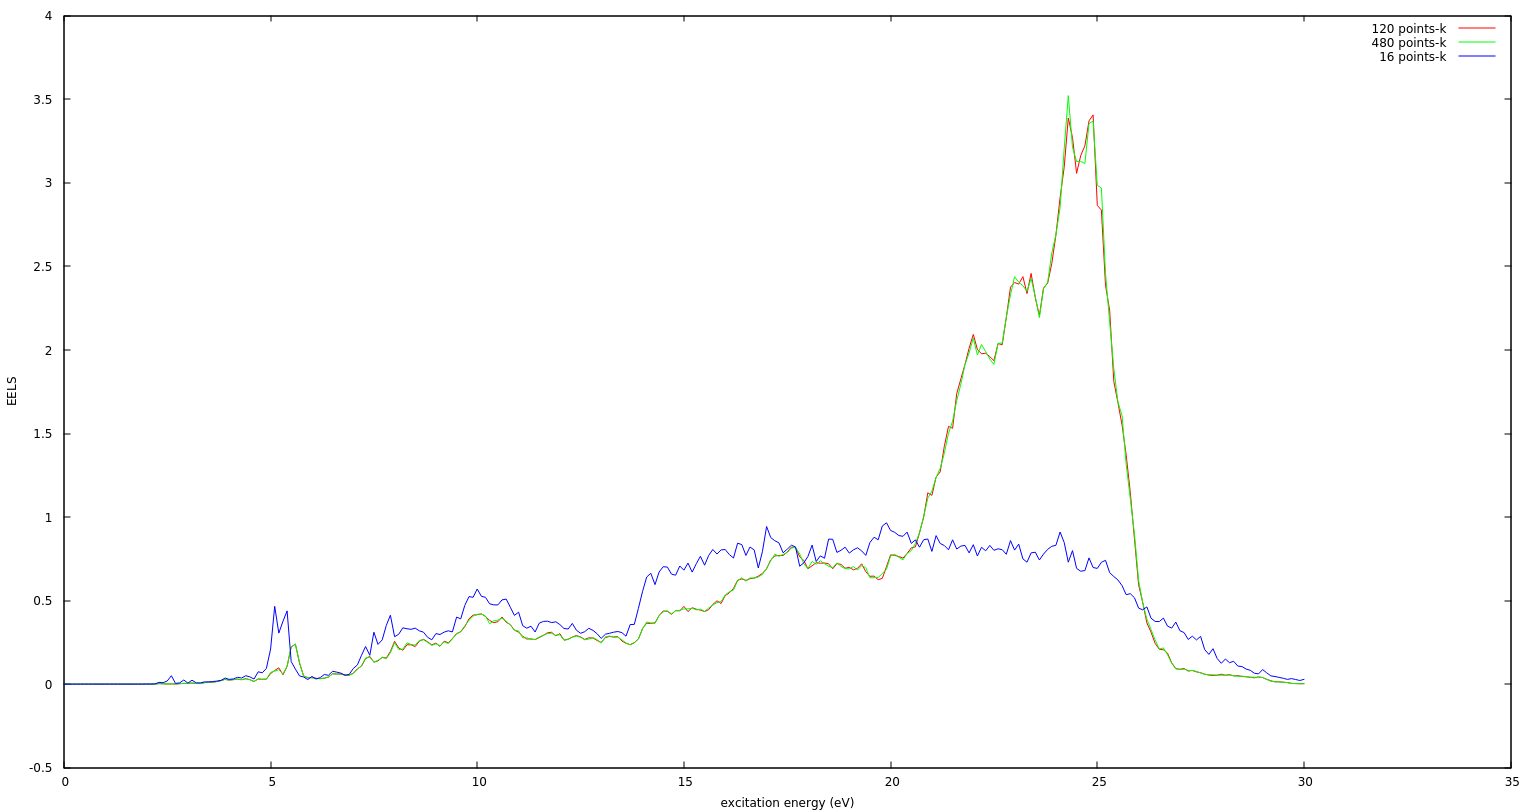
\includegraphics[width=\textwidth]{kpt_compare}
    \caption{Convergence pour des nombres de points-$\vb{k}$ différents}\label{fig-kptCompare}
\end{figure}

On montre dans la \cref{fig-kptCompare} que le choix du 120 points-$\vb{k}$ dans la première zone de Brillouin
donne déjà de bons résultats pour le calcul de EELS (par rapport à 480 points-$\vb{k}$).
On peut donc se contenter de prendre l'échantillonnage avec 120 points-$\vb{k}$ pour la suite.

\subsection{Convergence avec les bandes}
Pour le calcul de $\epsilon^{-1}$ (l'inverse de la fonction diélectrique, qui servira à calculer EELS),
il faut passer par le calcul de la fonction de polarisation $\chi^0$ (cf. \cref{chap-TRL}).
Pour ce calcul, on doit considérer toutes les transitions possibles
(excitation d'un électron de la bande de valence vers une bande de conduction).
Il est donc nécessaire de faire converger le calcul de EELS par rapport au nombre de bandes de valence
et de conduction (cf. \cref{eqn-chi}).
Le but est de considérer seulement les transitions pour les énergies qui nous intéressent
afin de gagner en temps de calcul sans perdre des informations.
Nous nous intéressons notamment aux transitions à basse énergie (< 20 eV).
Par conséquent, nous avons fait des calculs de EELS en variant le nombre de bandes de valence et le nombre de bandes de conduction.
Le résultat montré dans la \cref{fig-cv_nbd} montre qu'il suffit de prendre en compte
les transitions entre 46 bandes de valence et 92 bandes de conduction pour avoir le comportement du matériau pour la plage d'énergie qui nous intéresse.\footnote{
En effet, par l'étude de l'état fondamental, on sait qu'il y a un grand écart d'énergie entre la quarante-sixième et la quarante-septième bande de valence en comptant à partir de la surface de Fermi du matériau.}
\begin{figure}[!h]
    \centering
    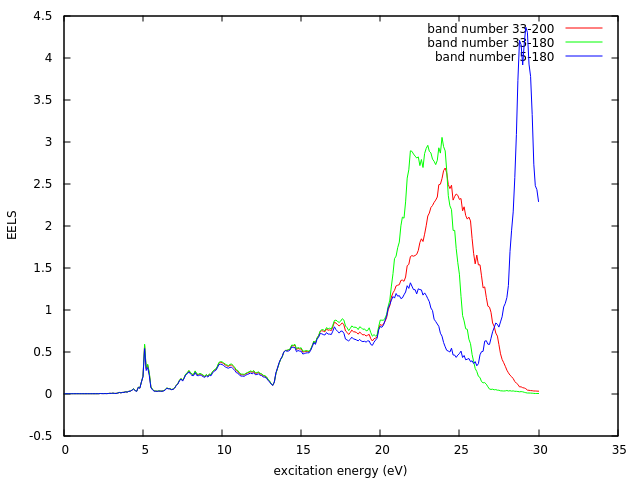
\includegraphics[width=\textwidth]{nbd_compare}
    \caption{Convergence en bande}\label{fig-cv_nbd}
\end{figure}

\subsection{RPA vs ALDA}
La méthode RPA prend moins de temps
pour le calcul mais pourrait perdre la précision.
Il est donc judicieux de comparer ces résultats obtenus avec ceux obtenus
en appliquant ALDA (adiabatic local density approximation).
On voit dans la \cref{fig-alda_vs_rpa} que
les deux approximations nous donnent des résultats assez proches à basse énergie.
Dans le cadre de ce projet, on se contente d'étudier les caractéristiques
de l'oxalate de calcium à basse énergie.
Il est donc tout à fait pertinent de faire nos calculs en RPA pour gagner en temps de calcul.
\begin{figure}[!h]
    \centering
    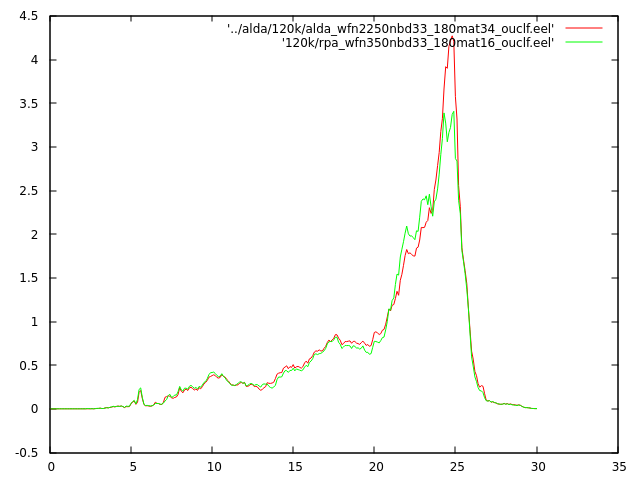
\includegraphics[width=\textwidth]{alda_vs_rpa}
    \caption{alda}\label{fig-alda_vs_rpa}
\end{figure}
\clearpage

\subsection{Anisotropie du système}
Cette étude consiste à examiner l'isotropie du système.
En effet, les transitions peuvent avoir lieu dans les directions différentes.
Un électron peut changer son vecteur d'onde en allant d'une bande à une autre.
Ce type de transition est pris en compte dans l'\cref{eqn-chi_q} qui nous donne la polarizabilité
que l'on est censé mesurer dans une direction donnée ($\vb{q}$ dans l'\cref{eqn-chi_q}).
Or, même à $\vb{q}$ petit, les fonctions de polarisabilité pour $\vb{q}$ de directions différentes peuvent être distinctes.
Les calculs de EELS en $\vb{q} = 0$ selon les trois axes
(par exemple, $\vb{q}=(0+,0,0)$ pour le premier axe de la zone de Brillouin)
sont montrés dans la \cref{fig-anisotropie}.
La différence entre les valeurs trouvées est dûe à l'anisotropie de la structure.

\begin{figure}[!h]
    \centering
    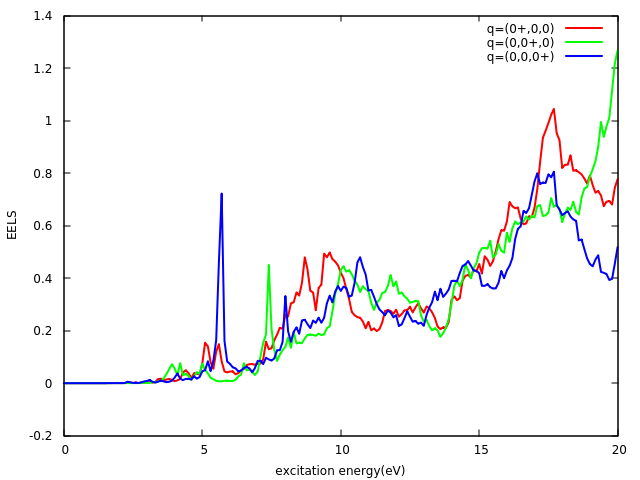
\includegraphics[width=\textwidth]{anisotropy}
    \caption{L'anisotropie du système}\label{fig-anisotropie}
\end{figure}

\subsection{EELS et la fonction diélectrique}
On se rappelle que la relation entre EELS et la fonction diélectrique est donnée par l'\cref{eqn-EELS}.
On peut constater que, dans la \cref{fig-epsilon_compare}, la partie réelle et
la partie imaginaire de la fonction diélectrique ont des sens de croissance opposés.
On pourrait donc s'attendre à un pic de résonance de EELS à l'endroit où elles se croisent
(aux alentours de 5 eV).
Ensuite, les deux parties prennent des valeurs bien supérieures à zéro,
la croissance de EELS dépend cette fois-ci plus de la partie imaginaire de la fonction diélectrique.
Le continuum du spectre pour le régime d'énergie supérieure à 7 eV est dû au fait
qu'il n'y a pas de croisement entre les parties réelle et imaginaire à valeur près de zéro.

\begin{figure}[!h]
    \centering
    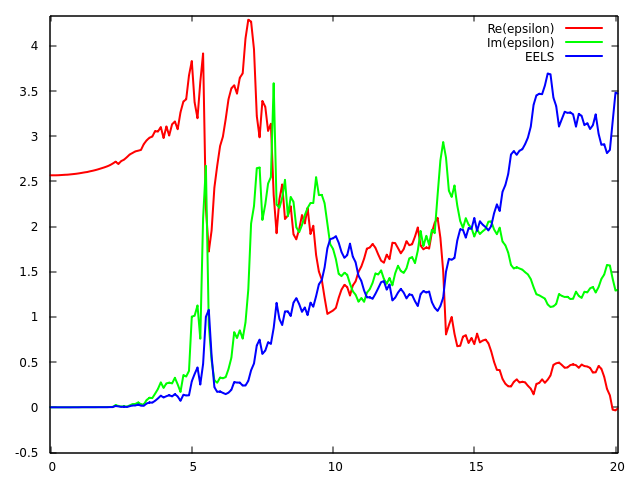
\includegraphics[width=\textwidth]{epsilon_compare}
    \caption{Relation entre les parties réelle et imaginaire\\ de la fonction diélectrique $\epsilon$ et EELS}\label{fig-epsilon_compare}
\end{figure}
\clearpage

\subsection{Dispersion}
Enfin, nous nous intéressons à la dispersion des spectres EELS\@.
Il s'agit de changer la valeur de $\vb{q}$ dans l'\cref{eqn-chi_q} (non proche de 0 cette fois-ci).
Il est intéressant de remarquer que la stabilité de la position du premier pique de résonance
pour les trois directions de dispersion différentes(cf. \cref{fig-q6,fig-q8,fig-q10}).
Bien que la valeur de EELS obtenue pour le premier pique change en fonction de $\vb{q}$,
le pique se trouve toujours en même énergie d'excitation
quand on fait varier la valeur de $\vb{q}$ dans une direction donnée.

Dans une vraie expérience, on est limité par la résolution des appareils.
Il est donc difficile à déterminer, en général, si une réponse forte est due
à une résonance ou à une superposition de réponses pour des valeurs de $\vb{q}$ différente.
Pour l'oxalate de calcium, un expérimentateur pourra se convaincre que la réponse qu'il obtient
pour une énergie qui correspond à un pique de EELS est une vraie résonance.

\begin{figure}[!b]
    \centering
    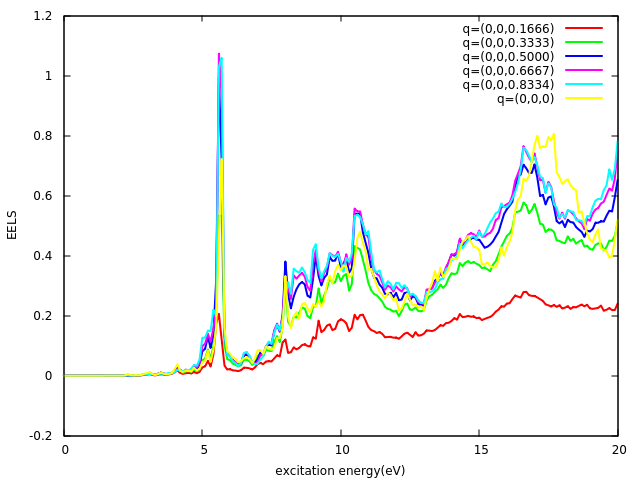
\includegraphics[height=0.4\textheight]{q6}
    \captionsetup{width=0.6\textwidth}
    \caption{EELS pour différents $\vb{q}$ dans la direction (0, 0, 1) dans la première zone de Brillouin}\label{fig-q6}
\end{figure}
\clearpage
\begin{figure}[!htb]
    \centering
    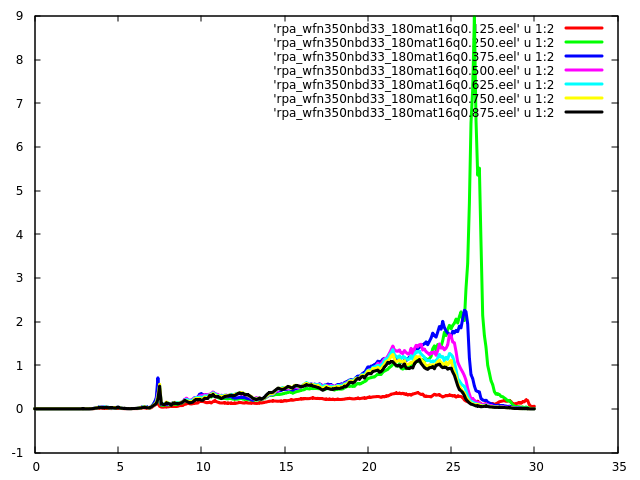
\includegraphics[height=0.4\textheight]{q8}
    \captionsetup{width=0.6\textwidth}
    \caption{EELS pour différents $\vb{q}$ dans la direction (0, 1, 0) dans la première zone de Brillouin}\label{fig-q8}
\end{figure}

\begin{figure}[!htb]
    \centering
    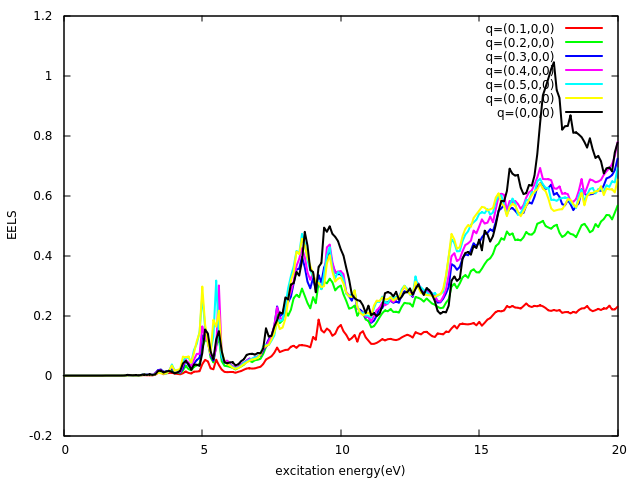
\includegraphics[height=0.4\textheight]{q10}
    \captionsetup{width=0.6\textwidth}
    \caption{EELS pour différents $\vb{q}$ dans la direction (1, 0, 0) dans la première zone de Brillouin}\label{fig-q10}
\end{figure}
